\documentclass[a4paper,12pt]{article}

\usepackage[spanish, activeacute]{babel} 
\usepackage{amsmath}
\usepackage{amsfonts}
\usepackage{amssymb}
\usepackage{graphicx}

\begin{document}

\tableofcontents
\pagebreak

\section{Autorizaci'on}

\pagebreak

\section{Resumen}

\pagebreak

\section{Palabras clave}

\pagebreak

\section{Introducci'on}

\pagebreak

\section{Especificaci'on de requisitos}

	\subsection{Descripci'on general}

	\subsection{Requisitos de interfaces externas}

	\subsection{Requisitos no funcionales}

	\subsection{Requisitos funcionales}

	\subsection{Coste econ'omico}

\pagebreak

\section{Casos de uso}

	\subsection{Inicio de sesi'on}
		\emph{\underline{Objetivo:}}\bigskip \\Se inicia la sesi\'on con el PDA abri\'endose as\'i la aplicaci\'on. Al iniciar la sesi\'on ser\'a necesario que el usuario introduzca su clave y nombre de usuario, que de ser correctos le dar\'an acceso a los men\'us.\bigskip \\ \emph{\underline{Entradas:}}
\begin{itemize}
\item Clave de usuario.
\item Nombre de usuario.
\end{itemize}
\emph{\underline{Precondiciones:}}\bigskip \\No hay precondiciones.\bigskip \\ \emph{\underline{Salidas:}}\bigskip \\En caso de \'exito (clave y nombre de usuario son correctos): 
\begin{itemize}
	\item Se muestra el men\'u de la aplicaci\'on en la pantalla del PDA.
\end{itemize}
En caso de fallo (clave y nombre de usuario no son correctos): 
\begin{itemize}
	\item Se informa al usuario de que los datos introducidos no son correctos.
	\item Se vuelve a la pantalla de inicio para que el usuario tenga la posibilidad de volver  a intentar iniciar la sesi'on.
\end{itemize}
\emph{\underline{Postcondici\'on si \'exito (clave y nombre de usuario son correctos):}}\bigskip \\Se muestra el men\'u de la aplicaci\'on por la pantalla del PDA.\bigskip \\ \emph{\underline{Postcondici\'on si fallo (clave y nombre de usuario no son correctos):}}\bigskip \\ Se informa al usuario de que los datos introducidos no son correctos y se le ofrece la posibilidad de intentar acceder a la aplicaci\'on de nuevo.\bigskip \\ \emph{\underline{Actores: }}
\begin{itemize}
	\item Usuario con PDA.
	\item Servidor del hospital.
	\item PDA.
\end{itemize}

\emph{\underline{Secuencia normal:}}
\begin{enumerate}
	\item Al encender el PDA, se solicita al usuario que introduzca su clave y su nombre de usuario y \'estos son enviados a la base de datos del servidor del hospital para que sean verificados.
	\item El servidor busca en su base de datos la clave y el nombre de usuario que se acaban de introducir para confirmar que est\'a iniciando sesi\'on una persona autorizada, personal del hospital. En caso de que la b\'usqueda tenga \'exito pasar a 3, en caso contrario pasar a E1.
	\item Una vez confirmada la clave y el nombre de usuario, en el PDA tenemos disponible el men\'u con todas las posibles operaciones que se pueden realizar con la aplicaci\'on.
\end{enumerate}

\emph{\underline{Secuencias alternativas:}}\bigskip \\ E1.- Se informa al usuario de que los datos que ha introducido no son correctos y se le da la oportunidad de volver a introducirlos (paso 1). \bigskip \\ Para ilustrar mejor est'a secuencia de acciones, incluimos el diagrama de secuencia de este caso de uso (Figura \ref{fig:inicio_sesion})

\begin{figure}[thb]
	\begin{center}
		\framebox{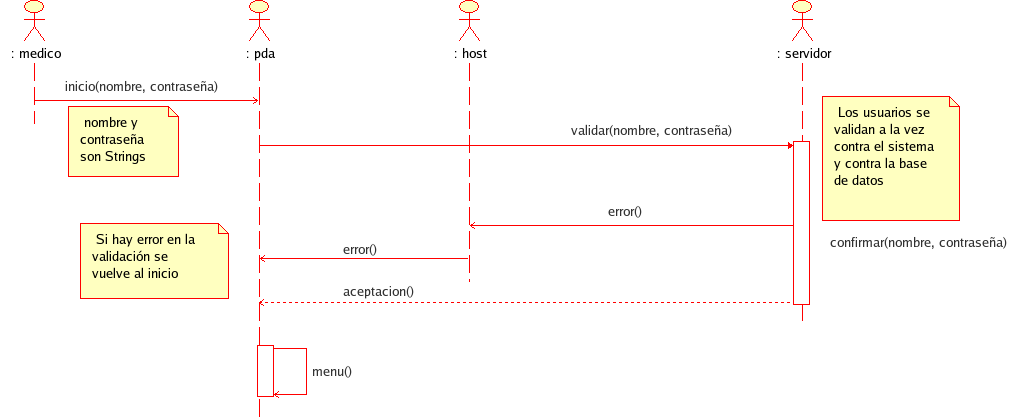
\includegraphics[scale=0.4]{dsecuenciainicio.png}}
     	\end{center}
    	\caption{Diagrama de secuencia del inicio de sesi'on}\label{fig:inicio_sesion}
\end{figure}

	\subsection{Impresi'on de documentos}
		\emph{\underline{Objetivo:}}\bigskip \\ El personal sanitario, dotado de un PDA, solicita la impresi\'on de un documento de un paciente que se encuentre disponible en la base de datos del hospital. Dicha impresi\'on se realizar'a por la impresora m\'as cercana al lugar en el que se ha solicitado \'esta.\bigskip \\ \emph{\underline{Entradas:}} 
\begin{itemize}
\item Documento a imprimir.
\item Nombre del paciente del que solicitamos el documento a imprimir.
\end{itemize}

\emph{\underline{Precondiciones:}}\bigskip \\ Los documentos que se solicitan imprimir deben encontrarse en la base de datos del hospital as'i como el paciente, que tambi'en debe estar registrado en la base de datos.\bigskip \\ \emph{\underline{Salidas:}}\bigskip \\ En caso de \'exito: 
\begin{itemize}
	\item Confirmaci\'on de la solicitud aceptada.
	\item Impresora por la que se va a realizar el trabajo.
	\item Documento imprimido en la impresora indicada.
\end{itemize}
En caso de fallo: 
\begin{itemize}
	\item Se informa al usuario de la imposibilidad de realizar la petici\'on.
\end{itemize}

\emph{\underline{Postcondici\'on si \'exito:}}\bigskip \\ Se realiza la impresi\'on por la impresora m\'as cercana.\bigskip \\ \emph{\underline{Postcondici\'on si fallo:}}\bigskip \\ Se informa de que no se ha podido realizar la impresi\'on y se vuelve al men'u principal.\bigskip \\ \emph{\underline{Actores: }}
\begin{itemize}
\item Usuario con PDA.
\item Servidor del hospital.
\item Cola de impresi\'on de las impresoras del centro.
\item PDA.
\end{itemize}

\emph{\underline{Secuencia normal:}} 
\begin{enumerate}
\item El usuario solicita al servidor la impresi\'on de un documento concreto de un paciente del hospital desde su PDA. Si error al conectar con el servidor pasa a E1, sino pasa a 2.
\item El servidor busca en su base de datos el documento que queremos imprimir. Si lo encuentra pasa a 3, sino pasa a E1.
\item El servidor calcula la posici\'on del PDA y en funci\'on de ella devuelve la impresora m'as cercana,  la elegida para imprimir el documento.
\item El servidor manda el documento a la cola de la impresora m\'as cercana.
\item El servidor envia al PDA la confirmaci\'on de impresi\'on aceptada, informando de cual es la impresora que en la que se realiza la tarea.
\item Volvemos al men'u principal.
\end{enumerate}

\emph{\underline{Secuencias alternativas:}}\bigskip \\E1.- Se informa al usuario de que no se puede realizar la impresi'on en ese momento y se le invita a intentarlo m\'as tarde. Volvemos al men'u principal.\bigskip \\ Para ilustrar mejor est'a secuencia de acciones, incluimos el diagrama de secuencia de este caso de uso (Figura \ref{fig:cu_imprimir})

\begin{figure*}[h!]
	\begin{center}
        		\framebox{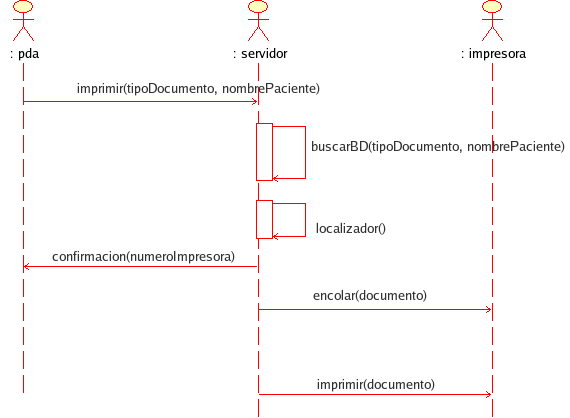
\includegraphics[scale=0.4]{dsecuenciaimprimir.png}}
     	\end{center}
    	\caption{Diagrama de secuencia de impresi'on de documentos}\label{fig:cu_imprimir}
\end{figure*}

	\subsection{Consulta de expedientes}
		\emph{\underline{Objetivo:}}\bigskip \\ Visualizaci'on por la pantalla del PDA del expediente de un paciente del hospital.\bigskip \\ \emph{\underline{Entradas:}}
\begin{itemize}
\item Nombre del paciente del que queremos consultar el expediente.
\end{itemize}

\emph{\underline{Precondiciones:}}\bigskip \\ El propietario del expediente que queremos visualizar debe ser un paciente registrado en la base de datos del hospital.\bigskip \\ \emph{\underline{Salidas:}}\bigskip \\ En caso de \'exito (el nombre paciente se encuentra en la base de datos del hospital): 
\begin{itemize}
	\item Se muestra en la pantalla del PDA el expediente del paciente solicitado.
\end{itemize}

En caso de fallo (el nombre paciente no se encuentra en la base de datos del hospital): 
\begin{itemize}
	\item Se informa al usuario de la imposibilidad de visualizar la informaci'on solicitada.
	\item Se vuelve al men'u principal.
\end{itemize}

\emph{\underline{Postcondici\'on si \'exito (el nombre paciente se encuentra en la base de datos del hospital):}}\bigskip \\ Se muestra el expediente del paciente solicitado en la pantalla del PDA.\bigskip \\ \emph{\underline{Postcondici\'on si fallo (el nombre paciente no se encuentra en la base de datos del hospital):}}\bigskip \\ Se informa al usuario de la imposibilidad de visualizar los datos solicitados y se vuelve al men'u principal.\bigskip \\ \emph{\underline{Actores: }}
\begin{itemize}
	\item Usuario con PDA.
	\item Servidor del hospital.
	\item PDA.
\end{itemize}

\emph{\underline{Secuencia normal:}}
\begin{enumerate}
	\item El usuario solicita al servidor la consulta del expediente de un paciente del hospital desde su PDA.
	\item El servidor busca en su base de datos el expediente del paciente solicitado. En caso de que la b\'usqueda tenga \'exito pasar a 3, en caso contrario pasar a E1.
	\item Se hace una lectura del expediente solicitado y se env'ia al PDA, mostr'andose por pantalla.
	\item Volvemos al men'u principal.
\end{enumerate}

\emph{\underline{Secuencias alternativas:}}\bigskip \\ E1.- Se informa al usuario del error en la consulta y se vuelve al men'u principal.\bigskip \\ Para ilustrar mejor est'a secuencia de acciones, incluimos el diagrama de secuencia de este caso de uso (Figura \ref{fig:consulta_expediente})

\begin{figure*}[h!]
	\begin{center}
        		\framebox{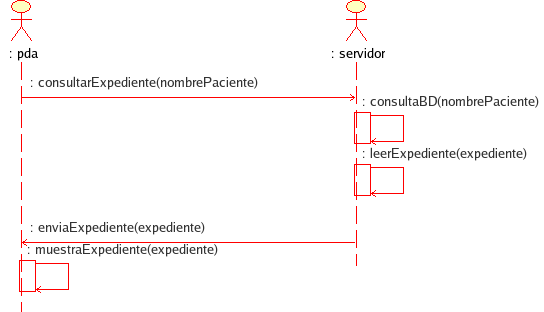
\includegraphics[scale=0.4]{consultar_expediente.png}}
     	\end{center}
    	\caption{Diagrama de secuencia de consultar expediente}\label{fig:consulta_expediente}
\end{figure*}		

\pagebreak

\section{Implementaci'on}

	\subsection{Tecnolog'ias}
		\begin{itemize}
\item J2ME:\bigskip \\Java 2 Micro Edition (J2ME), es un subconjunto de J2SE orientado al desarrollo de aplicaciones Java destinadas a dispositivos con capacidades restringidas, tanto con respecto a la capacidad de memoria disponible, limitaciones de memoria gr'afica como con respecto a la capacidad de procesamiento, en nuestro caso, un PDA.\bigskip \\Hay varias formas de implementar aplicaciones del tipo que estamos presentado.\bigskip \\Por un lado, tenemos las aplicaciones ligeras, basadas en el mundo web. Utilizan lenguajes como WML o HTML para el desarrollo de contenidos y emplean el protocolo HTTP para comunicarse con un servidor que proporciona el contenido de el cliente debe presentar al usuario. El principal inveniente de estas aplicaciones es que el usuario tiene que estar continuamente conectado.\bigskip \\Por otro lado, est'an las aplicaciones nativas, que son aquellas desarrolladas para un sistema operativo determinado como PalmOS, Windows CE o EPOC y est'an escritas en lenguaje C/C++ o incluso  BASIC. Estas aplicaciones se pueden ejecutar de forma aut'onoma, sin necesidad de conexi'on, pero son totalmente dependientes del sistema operativo para el que han sido creadas.\bigskip \\Finalmente, J2ME auna lo mejor de los dos mundos y salva sus principales incovenientes al ser multiplataforma, importante inconveniente de las aplicaciones nativas, y al proporcionar todos los elementos de Java, como control de la persistencia, conexi'on a la red o interfaz de usuario, que no est'an disponibles en las aplicaciones ligeras.

\item XML-RPC:\bigskip \\Dada la naturaleza de la aplicaci'on, se hac'ia necesario el empleo de un protocolo de intercambio de informaci'on entre el PDA y el servidor del hospital. El protocolo XML-RPC es un protocolo extremadamente ligero para la invocaci'on de procesos remotos sobre una red enviando mensajes XML formateados sobre protocolo HTTP. \bigskip \\Aunque la especificaci'on de J2ME no proporciona soporte nativo para XML-RPC, el proyecto de c'odigo abierto kXML-RPC es una implementaci'on de XML-RPC destinada a dispositivos compatibles MIDP, basada en Kxml , con lo que empleando estas librer'ias ya ten'iamos solucionado el intercambio de informaci'on.\bigskip \\Otra posibilidad era emplear el protocolo Simple Object Access Protocol (SOAP). SOAP es un protocolo ligero de intercambio de informaci'on estructurada en un entorno descentralizado y distribuido. La idea subyace en la creaci'on de este protocolo es proporcionar un mecanismo uniforme para realizar llamadas a procedimientos remotos utilizando HTTP como protocolo de comunicaci'on y XML  como mecanismo de serializaci'on de datos.\bigskip \\XML-RPC y SOAP son protocolos muy similares pero SOAP ofrece una mayor versatilidad a cambio de una mayor sobrecarga. A la hora de la elecci'on ten'iamos que tener presente la escasez de memoria de los dispositivos compatibles J2ME, que el poder de procesamiento no es abundante y que el ancho de banda disponible en los dispositivos m'oviles no es demasiado grandey dado que SOAP proporciona propiedades extra que no eran necesarias para la aplicaci'on, la elecci'on autom'atica fue XML-RPC.

\item MySQL:\bigskip \\En la actualidad, hay muchos sistemas gestores de bases de datos, por ejemplo, Oracle o Microsoft Access. MySQL, es el sistema que hemos escogido para gestionar la base de datos del hospital. El motivo que nos ha impulsado a ello es que est'a desarrollado bajo la filosof'ia de c'odigo abierto y que es multiplataforma. Adem'as, J2SE cuenta con el paquete java.sql que proporciona numerosas utilidades para hacer consultas a bases de datos MySQL desde aplicaciones Java, lo que hace muy f'acil su integraci'on con el programa servidor del hospital.

\item Ubuntu Server:\bigskip \\ En el servidor hemos instalado Ubuntu server. Una variedad de Ubuntu para servidores. Ubuntu es una distribuci'on de Linux, basada en Debian. Sus principales caracter'isticas son:
\begin{enumerate}
	\item Se en la distribuci'on Debian.
	\item Está disponible para Intel x86, AMD64, PowerPC.
	\item El sistema incluye funciones avanzadas de seguridad y entre sus pol'iticas se encuentra el no activar procesos latentes por omisi'on al momento de instalarse. Por eso mismo, no hay un firewall predeterminado, ya que no existen servicios que puedan atentar a la seguridad del sistema.
\end{enumerate}

Ubuntu divide todo el software en cuatro secciones:
\begin{enumerate}
	\item main 
	\item estricted
	\item universe
	\item multiverse
\end{enumerate}

\item CUPS: \bigskip \\ Como servidor de impresi'on hemos usado Common Unix Printing System (CUPS). Es un sistema de impresi'on modular para sistemas de operativos unix. Permite que un computador act'ue como servidor de impresi'on. Un computador que ejecuta CUPS act'ua como un servidor que puede aceptar tareas de impresi'on desde otros computadores clientes, los procesa y los env'ia al servidor de impresi'on apropiado. \bigskip \\ CUPS est'a compuesto por una cola de impresi'on con su programaci'on, un sistema de filtros que convierte datos para imprimir hacia formatos que la impresora conozca, y un sistema de soporte que env'ia los datos al dispositivo de impresi'on. CUPS utiliza el protocolo IPP como base para el manejo de tareas de impresi'on y de colas de impresi'on. Tambi'en provee los comandos tradicionales de impresi'on de los sistemas Unix y un soporte limitado de operaciones bajo el protocolo SMP. Los programas de manejo de dispositivo de impresi'on que CUPS provee est'an basados en la Descripción de impresoras PostScript (PPD). Existen varias interfaces de usuario para diferentes plataformas para configurar CUPS, incluso una interfaz Web. CUPS se distribuye bajo licencia GNU General Public License y GNU Lesser General Public License, Versión 2.
\end{itemize}		

	\subsection{Dise'no}

\pagebreak

\section{An'alisis del sistema}

	\subsection{Triangulaci'on}

	\subsection{Algoritmo de Floyd}

	\subsection{Conexi'on PDA-Servidor}
		Las llamadas remotas a procedimientos del servidor del hospital (login, consultas a bases de datos...) que se hacen desde el PDA se llevan a cabo a trav'es del protocolo XML-RPC. \bigskip \\  Un mensaje XML-RPC se incrusta en una petici'on POST enviada por el PDA. El servidor del hospital recibe la petici'on, analiza el documento XML, ejecuta el procedimiento con los par'ametros adecuados y devuelve el resultado como un documento XML formateado al PDA mediante respuesta HTTP.\bigskip \\ Para ejemplificar este proceso, transcribimos los respectivos mensajes que se pasan servidor y PDA en el procedimiento de login, cuando queremos iniciar sesi'on con el PDA. \bigskip \\ Primero el PDA env'ia el nombre de usuario y la clave personal que ha introducido el m'edico al servidor del hospital para que contraste estos datos con la base de datos.

\begin{verbatim}
<methodCall>
 <methodName>bd.login</methodName>
 <params>
  <param>
   <value>
    <string>tablaMedicos</string>
   </value>
  </param>
  <param>
   <value>
    <string>HOUSE</string>
   </value>
  </param>
  <param>
   <value>
    <string>STACY</string>
   </value>
  </param>
 </params>
</methodCall>
\end{verbatim}

Una  vez que 'este ha ejecutado el procedimiento solicitado, el servidor env'ia la respuesta con el resultado al PDA:

\begin{verbatim}
<methodResponse>
 <methodName>bd.login</methodName>
 <params>
  <param>
   <value>
    <string>si</string>
   </value>
  </param>
 </params>
</methodResponse>
\end{verbatim}

	\subsection{Base de datos}
		Dado los escasos casos de uso que se han implementado a lo largo del proyecto, no se consider'o necesario una base de datos muy sofisticada. As'i creamos una base de datos ''Hospital'', con dos tablas, una para datos del personal del hospital, ''tablaMedicos'', y otra para datos de pacientes, ''tablaPacientes''.

\begin{verbatim}
+--------------------+
| Tables_in_Hospital |
+--------------------+
| tablaMedicos       |
| tablaPacientes     |
+--------------------+
\end{verbatim}

La tabla ''tablaMedicos'' tiene dos entradas, usuario y clave, correspondientes con los datos que tienen que introducir los m'edicos cada vez que quieren iniciar sesi'on en el PDA:

\begin{verbatim}
+---------+--------+
| USUARIO | CLAVE  |
+---------+--------+
| HOUSE   | STACY  |
| CAMERON | ISLA   |
| FOREMAN | CARCEL |
+---------+--------+
\end{verbatim}

La tabla ''tablaPacientes'' tiene tres entradas correspondientes con el nombre del paciente, la ruta en la que se encuentran almacenados en el servidor del hospital sus 'ultimos an'alisis y su expediente:

\begin{figure}[h]
	\begin{center}
		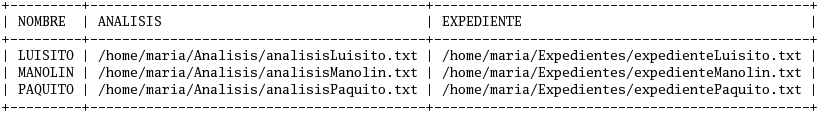
\includegraphics[scale=0.55]{bd.png}
     	\end{center}
\end{figure}

El servidor MySQL est'a continuamente funcinando en el servidor del hospital de manera que en cualquier momento son posibles los accesos a la base de datos tanto para login de los m'edicos con su PDA como para consulta de documentos de los pacientes. Estas consultas a la base de datos se hacen a trav'es de Java, gracias al paquete java.sql de J2SE.

\pagebreak

\section{Manual de usuario}
	\begin{enumerate}
\item Inicio de sesi'on: \newline
Cuando un m'edico enciende su PDA para empezar a trabajar, lo primero que se encuentra es con la pantalla Inicio de sesi'on. El m'edico deber'a introducir su nombre de usuario y su clave personal en los cuadros de texto correspondientes vali'endose del teclado del PDA y pulsar el bot'on Aceptar. Este es un procedimiento rutinario que impide que personal no autorizado pueda acceder a informaci'on confidencial del hospital.

%\begin{figure*}[h!]
%	\begin{center}
%        		\framebox{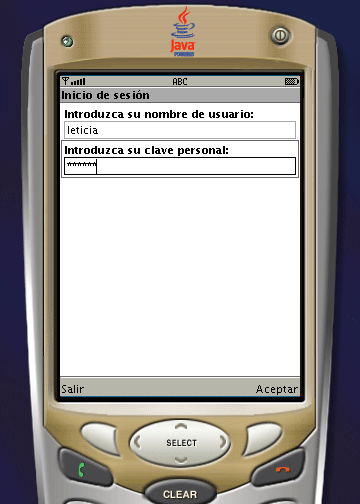
\includegraphics[width=1.0\textwidth]{inicio.png}}
%     	\end{center}
%    	\caption{Diagrama de secuencia del inicio de sesi'on}\label{fig:inicio_sesion}
%\end{figure*}

En caso de que el m'edico no haya introducido correctamente su nombre de usuario o su clave personal, no podr'a acceder a la aplicaci'on. Se le informar'a de ello y se le dar'a la oportunidad de introducir sus datos de nuevo.

%\begin{figure*}[h!]
%	\begin{center}
%        		\framebox{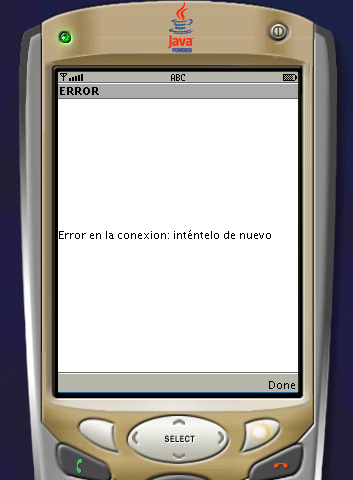
\includegraphics[width=1.0\textwidth]{error_inicio.png}}
%     	\end{center}
%    	\caption{Pantalla de error en el inicio de sesi'on}\label{fig:pantalla_error_inicio}
%\end{figure*}

En caso de que puls'aramos el bot'on Salir, en el margen inferior izquierdo de la pantalla, saldr'iamos de la aplicaci'on y se apagar'ia el PDA.

\item Men'u principal:\newline
Una vez iniciada la sesi'on, el m'edico tiene acceso al men'u principal donde se le ofertan todas las utilidades de la aplicaci'on.

%\begin{figure*}[h!]
%	\begin{center}
%        		\framebox{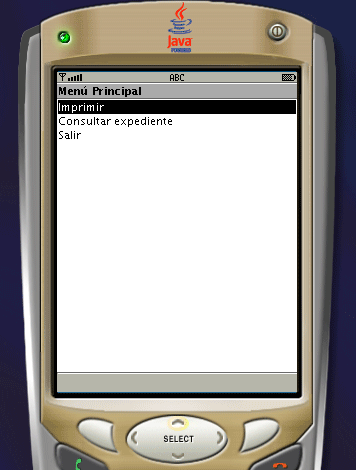
\includegraphics[width=1.0\textwidth]{menu_principal.png}}
%     	\end{center}
%    	\caption{Pantalla del men'u principal}\label{fig:pantalla_principal}
%\end{figure*}

Para elegir una opci'on del men'u debe desplazarse por el men'u con las flechas centrales hacia arriba y hacia abajo y pulsar Select cuando tenga seleccionada la tarea que desea realizar.

Ahora hablaremos de las diferentes opciones del men'u principal:
\begin{itemize}

\item Men'u de impresi'on:\newline
A trav'es de esta opci'on podemos imprimir un documento disponible del paciente del hospital deseado: s'olo tenemos que elegir el tipo de documento a imprimir (Expediente o 'Ultimos an'alisis) e introducir a trav'es del teclado el nombre del paciente del que precisamos los documentos. Una vez introducidos estos datos, solo hay que pulsar el bot'on Aceptar, en el margen inferior derecho de la pantalla.

%\begin{figure*}[h!]
%	\begin{center}
%        		\framebox{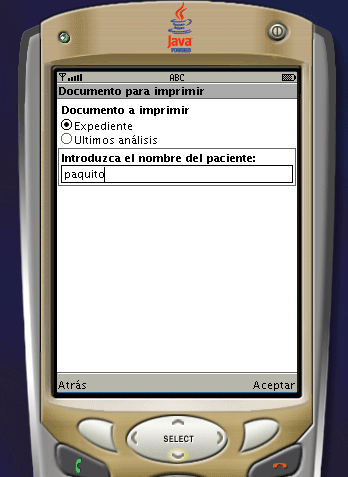
\includegraphics[width=1.0\textwidth]{menu_imprimir.png}}
%     	\end{center}
%    	\caption{Pantalla del men'u de impresi'on}\label{fig:pantalla_imprimir}
%\end{figure*}

El bot'on Atr'as nos devuelve al men'u principal.

En caso de que introduzcamos mal el nombre del paciente, no est'en disponibles los documentos o no sea posible el uso de las impresoras, se informar'a al usuario y se le instar'a a intentarlo m'as tarde.

%\begin{figure*}[h!]
%	\begin{center}
%        		\framebox{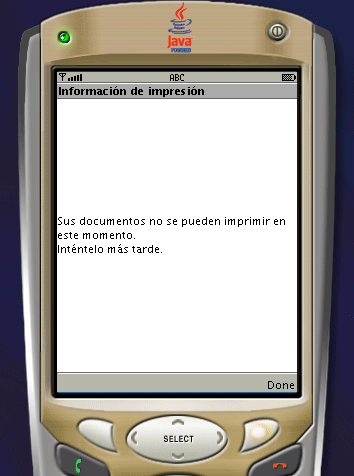
\includegraphics[width=1.0\textwidth]{error_imprimir.png}}
%     	\end{center}
%    	\caption{Pantalla de error en el procedimiento de imprimir}\label{fig:error_imprimir}
%\end{figure*}

En caso de que no haya ning'un problema en la realizaci'on  de la tarea, se informar'a al usuario de la impresora por la que se llevar'a a cabo la impresi'on solicitada.

%\begin{figure*}[h!]
%	\begin{center}
%        		\framebox{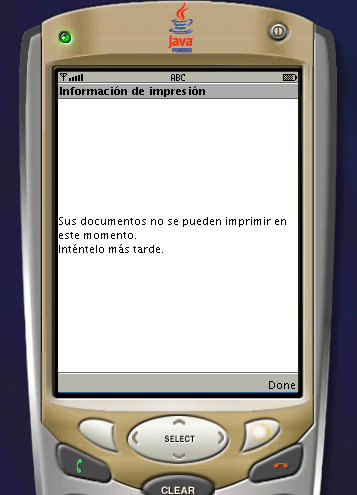
\includegraphics[width=1.0\textwidth]{acierto_imprimir.png}}
%     	\end{center}
%    	\caption{Pantalla de informaci'on de impresi'on}\label{fig:acierto_imprimir}
%\end{figure*}

\item Consultar expediente:\newline
Con esta opci'on podemos visualizar en la pantalla del PDA el expediente del paciente deseado. Al seleccionarla llegamos a  una pantalla en la solo tenemos que introducir el nombre del paciente y pulsar el bot'on Aceptar para acceder al expediente deseado.

%\begin{figure*}[h!]
%	\begin{center}
%        		\framebox{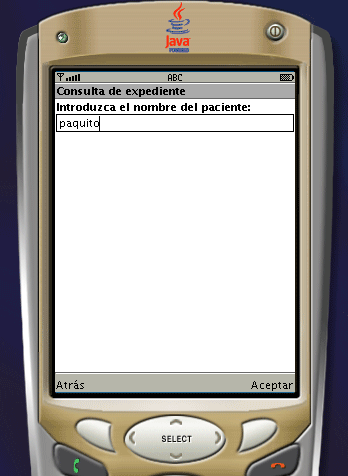
\includegraphics[width=1.0\textwidth]{menu_consulta.png}}
%     	\end{center}
%    	\caption{Pantalla de petici'on de consulta de expediente}\label{fig:menu_consulta}
%\end{figure*}

El bot'on Atr'as nos devuelve al men'u principal.

En caso de que introduzcamos mal el nombre del paciente o no est'en disponibles los documentos, se informar'a al usuario.

%\begin{figure*}[h!]
%	\begin{center}
%        		\framebox{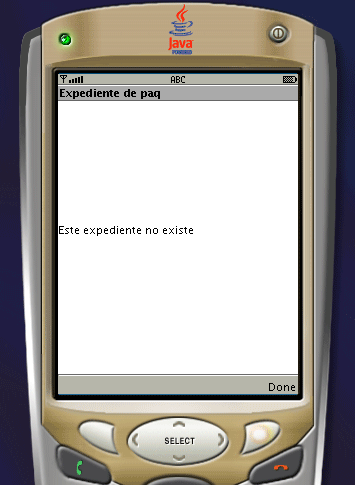
\includegraphics[width=1.0\textwidth]{error_consulta.png}}
%     	\end{center}
%    	\caption{Pantalla de error en la consulta de expediente}\label{fig:error_consulta}
%\end{figure*}

En caso de que los datos sean correctos se mostrar'a por pantalla el expediente del paciente solicitado.

%falta pantallazo de esto!!!!!!!!!!!!!!!!!!!!!!!!!!!!!

\item Salir:\newline
Esta opci'on nos permite salir de la aplicaci'on y apagar el PDA.
 
\end{itemize}


\end{enumerate}	

\pagebreak

\section{Valoraci'on}

\pagebreak

\section{Ap'endices}

	\subsection{J2ME}
		Como ya hemos comentado anteriormente, Java 2 Micro Edition (J2ME), es un subconjunto de J2SE orientado al desarrollo de aplicaciones Java destinadas a dispositivos con capacidades restringidas. \bigskip \\ La arquitectura J2ME est'a dise'nada con la filosof'ia de ser escalable y modular, ya que no se conoce como ser'an los dispositivos en el futuro y debe estar preparada para adaptarse a ellos. Sus caracter'isticas est'an definidas en un entorno global constituido por varias capas, de abajo a arriba:

\begin{enumerate}
\item Capa correspondiente a la M'aquina Virtual de Java: una versi'on reducida para dispositivos reducidos.
\item Capa de Configuraci'on: est'a orientada al dispositivo y define el m'inimo conjunto de caracter'isticas de la m'aquina virtual Java y de las librer'ias de clases Java que est'an disponibles para un conjunto de dispositivos.
\item Capa de Perfil: est'a orientada a la aplicaci'on y define el m'inimo conjunto de APIs disponibles para una determinada familia de dispositivos. Entre los perfiles que se han desarrollado hasta ahora, destaca el perfil PDA, que extiende el perfil CLDC para adecuarse a las ventajas que ofrecen los dispositivos PDA.
\item Capa del \textit{Perfil para Dispositivos de Informaci'on M'ovil} (MIDP) consiste en un conjunto de APIs Java que permiten la creaci'on de interfaces de usuario, conexiones de red, manipulaci'on de datos, sonido, seguridad...
\end{enumerate}

La combinaci'on de las tres primeras capas constituye la configuraci'on CLDC, que junto con la capa MIDP forman el entorno de ejecuci'on est'andar pra las aplicaciones y servicios que se pueden descargar din'amincamente sobre los dispositivos de los usuarios finales, como pueden ser los PDA. \bigskip \\ El coraz'on del perfil MIDP es un \textbf{midlet}. Una aplicaci'on midlet extiende la clase MIDlet, que proporciona a esa aplicaci'on la posibilidad de recuperar propiedades, controlar cambios de estado y constituye la interfaz entre el entorno de ejecuci'on del dispositivo y el c'odigo de la aplicaci'on midlet.\bigskip \\ El hecho de que una aplicaci'on midlet extienda la clase MIDlet hace que el programador se vea obligado a implementar los siguiente m'etodos abstractos:

\begin{itemize}
\item starApp(): en este m'etodo la aplicaci'on hace acopio de los recursos que va a necesitar el midlet y donde se preparan los controladores de eventos.
\item pauseApp(): este m'etodo es invocado cuando se necesita detener la ejecuci'on del midlet temporalmente.
\item destroyApp(): este m'etodo es invocado cuando el midlet debe ser destruido o tambi'en puede ser invocado por el propio midlet antes de finalizar su ejecuci'on.
\end{itemize}

La implementaci'on de estos m'etos asegura que el midlet pueda pasar por todos los estados de su ciclo de vida: DETENIDO, ACTIVO, DESTRUIDO.

	%\subsection{XML-RPC}

	\subsection{Algoritmo de Floyd}

\pagebreak

\begin{thebibliography}{XXX}

	\bibitem{Froute}J2ME Java 2 Micro Edition. Manual de usuario y tutorial.Agust'in Froute Quintas, Patricia Jorge C'ardenes. Ed. Ra-Ma.
	\bibitem{sun}http://java.sun.com
	\bibitem{kxmlrpc}http://kxmlrpc.objectweb.org
	\bibitem{eclipseme}  http://eclipseme.sourceforce.net
	\bibitem{wikipedia} http://es.wikipedia.org
	%\bibitem{mysql}http://www.programacion.com/bbdd/tutorial/mysql_basico

\end{thebibliography}

\end{document}